\PassOptionsToPackage{unicode=true}{hyperref} % options for packages loaded elsewhere
\PassOptionsToPackage{hyphens}{url}
%
\documentclass[ignorenonframetext,]{beamer}
\usepackage{pgfpages}
\setbeamertemplate{caption}[numbered]
\setbeamertemplate{caption label separator}{: }
\setbeamercolor{caption name}{fg=normal text.fg}
\beamertemplatenavigationsymbolsempty
\usepackage{lmodern}
\usepackage{amssymb,amsmath}
\usepackage{ifxetex,ifluatex}
\usepackage{fixltx2e} % provides \textsubscript
\ifnum 0\ifxetex 1\fi\ifluatex 1\fi=0 % if pdftex
  \usepackage[T1]{fontenc}
  \usepackage[utf8]{inputenc}
  \usepackage{textcomp} % provides euro and other symbols
\else % if luatex or xelatex
  \usepackage{unicode-math}
  \defaultfontfeatures{Ligatures=TeX,Scale=MatchLowercase}
\fi
\usetheme[]{Copenhagen}
\usecolortheme{wolverine}
% use upquote if available, for straight quotes in verbatim environments
\IfFileExists{upquote.sty}{\usepackage{upquote}}{}
% use microtype if available
\IfFileExists{microtype.sty}{%
\usepackage[]{microtype}
\UseMicrotypeSet[protrusion]{basicmath} % disable protrusion for tt fonts
}{}
\IfFileExists{parskip.sty}{%
\usepackage{parskip}
}{% else
\setlength{\parindent}{0pt}
\setlength{\parskip}{6pt plus 2pt minus 1pt}
}
\usepackage{hyperref}
\hypersetup{
            pdftitle={HPC},
            pdfauthor={JCN-9000},
            pdfborder={0 0 0},
            breaklinks=true}
\urlstyle{same}  % don't use monospace font for urls
\newif\ifbibliography
\usepackage{longtable,booktabs}
\usepackage{caption}
% These lines are needed to make table captions work with longtable:
\makeatletter
\def\fnum@table{\tablename~\thetable}
\makeatother
\usepackage{graphicx,grffile}
\makeatletter
\def\maxwidth{\ifdim\Gin@nat@width>\linewidth\linewidth\else\Gin@nat@width\fi}
\def\maxheight{\ifdim\Gin@nat@height>\textheight\textheight\else\Gin@nat@height\fi}
\makeatother
% Scale images if necessary, so that they will not overflow the page
% margins by default, and it is still possible to overwrite the defaults
% using explicit options in \includegraphics[width, height, ...]{}
\setkeys{Gin}{width=\maxwidth,height=\maxheight,keepaspectratio}
% Prevent slide breaks in the middle of a paragraph:
\widowpenalties 1 10000
\raggedbottom
\setbeamertemplate{part page}{
\centering
\begin{beamercolorbox}[sep=16pt,center]{part title}
  \usebeamerfont{part title}\insertpart\par
\end{beamercolorbox}
}
\setbeamertemplate{section page}{
\centering
\begin{beamercolorbox}[sep=12pt,center]{part title}
  \usebeamerfont{section title}\insertsection\par
\end{beamercolorbox}
}
\setbeamertemplate{subsection page}{
\centering
\begin{beamercolorbox}[sep=8pt,center]{part title}
  \usebeamerfont{subsection title}\insertsubsection\par
\end{beamercolorbox}
}
\AtBeginPart{
  \frame{\partpage}
}
\AtBeginSection{
  \ifbibliography
  \else
    \frame{\sectionpage}
  \fi
}
\AtBeginSubsection{
  \frame{\subsectionpage}
}
\setlength{\emergencystretch}{3em}  % prevent overfull lines
\providecommand{\tightlist}{%
  \setlength{\itemsep}{0pt}\setlength{\parskip}{0pt}}
\setcounter{secnumdepth}{0}

% set default figure placement to htbp
\makeatletter
\def\fps@figure{htbp}
\makeatother


\title{HPC}
\author{JCN-9000}
\date{2019-05-20}

\begin{document}
\frame{\titlepage}

\begin{frame}{HPC}

\begin{itemize}
\item
  High Performance Computer : Supercomputer
\item
  High Performance Computing : Parallel
\item
  \href{https://boinc.berkeley.edu/}{BOINC} is a platform for
  high-throughput computing "Seti@Home", "Folding@Home", (
  \href{https://en.wikipedia.org/wiki/List_of_distributed_computing_projects}{List
  of distributed computing projects} )
\end{itemize}


\end{frame}

\begin{frame}{Definition}

\begin{description}
\tightlist
\item[\href{https://insidehpc.com/hpc-basic-training/what-is-hpc/}{HPC}]
High Performance Computing most generally refers to the practice of
aggregating computing power in a way that delivers much higher
performance than one could get out of a typical desktop computer or
workstation in order to solve large problems in science, engineering, or
business.
\end{description}

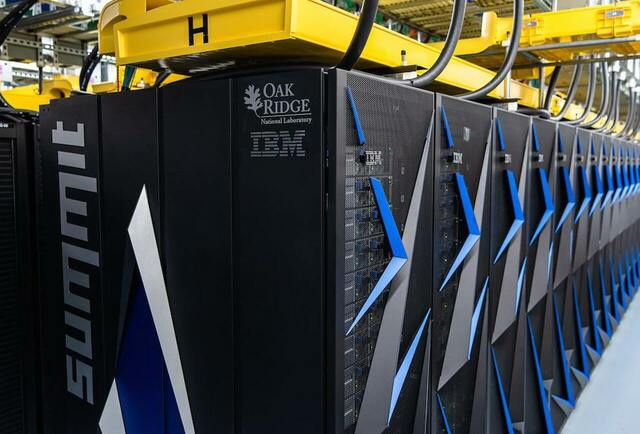
\includegraphics{images/Summit_small.jpg} :

\end{frame}

\begin{frame}{Wikipedia IT}

\begin{description}
\tightlist
\item[\href{https://it.wikipedia.org/wiki/High_Performance_Computing}{HPC}]
Con High Performance Computing (HPC) (in italiano calcolo ad elevate
prestazioni), in informatica, ci si riferisce alle tecnologie utilizzate
da computer cluster per creare dei sistemi di elaborazione in grado di
fornire delle prestazioni molto elevate nell'ordine dei PetaFLOPS,
ricorrendo tipicamente al calcolo parallelo.
\end{description}


\end{frame}

\begin{frame}{FLOPS}

\begin{itemize}
\tightlist
\item
  FLOPS Unit \url{https://en.wikipedia.org/wiki/Unit_prefix}
\end{itemize}


\begin{longtable}[]{@{}llll@{}}
\toprule
\endhead
& & \textbf{Metric prefixes in everyday use} &\tabularnewline
Text & Symbol & Factor & Power\tabularnewline
yotta & Y & 1000000000000000000000000 & 10E24\tabularnewline
zetta & Z & 1000000000000000000000 & 10E21\tabularnewline
exa & E & 1000000000000000000 & 10E18\tabularnewline
peta & P & 1000000000000000 & 10E15\tabularnewline
tera & T & 1000000000000 & 10E12\tabularnewline
giga & G & 1000000000 (PC) & 10E9\tabularnewline
mega & M & 1000000 & 10E6\tabularnewline
kilo & k & 1000 & 10E3\tabularnewline
hecto & h & 100 & 10E2\tabularnewline
deca & da & 10 & 10E1\tabularnewline
(none) & (none) & 1 & 10E0\tabularnewline
\bottomrule
\end{longtable}

\end{frame}

\begin{frame}[fragile]{Local FLOPS using HPL/Linpak}

\begin{itemize}
\tightlist
\item
  \href{http://hpl-calculator.sourceforge.net/}{Rate Your PC}
\end{itemize}

\begin{block}{Netlib Linpak}

\begin{itemize}
\tightlist
\item
  HPL from Netlib
\item
  \url{http://www.netlib.org/benchmark/hpl/}
\item
  \href{https://www.advancedclustering.com/act_kb/tune-hpl-dat-file/}{Build
  HPL.dat}
\end{itemize}

\begin{verbatim}
cd ~/GIT/Polito-HPC/hpl-2.3/testing
mpirun -np 2 ./xhpl
\end{verbatim}

\end{block}

\begin{block}{Intel Linpak}


\begin{enumerate}
\tightlist
\item
  Download Intel Linpak
  \href{https://software.intel.com/en-us/articles/intel-mkl-benchmarks-suite}{(link)}
\item
  Extract
\item
  cd .../linux/mkl/benchmarks/linpack
\item
  ./runme\_xeon64
\end{enumerate}

\begin{verbatim}
cd ~/GIT/Polito-HPC/l_mklb_p_2018.3.011
cd benchmarks_2018/linux/mkl/benchmarks/linpack
./runme_xeon64
\end{verbatim}

+

\end{block}

\end{frame}

\begin{frame}[fragile]{TOP\_500}

\begin{itemize}
\tightlist
\item
  TOP\_500 \url{https://www.top500.org/}
\item
  \href{https://www.top500.org/lists/2018/11/}{1-10 LIST}
\item
  \href{https://www.top500.org/list/2018/11/?page=1}{1-100}
\end{itemize}

\begin{verbatim}
\end{verbatim}

\href{https://www.eni.com/it_IT/innovazione/piattaforme-tecnologiche/aumento-recupero-idrocarburi/hpc.page}{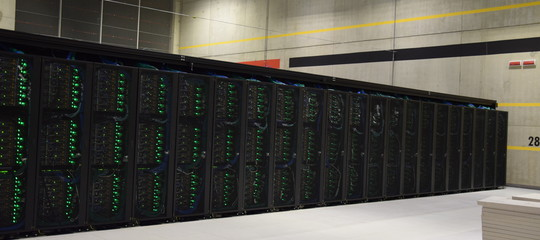
\includegraphics{images/HPC4-ENI.jpg}}

\end{frame}

\begin{frame}{Hardware components}

\begin{itemize}
\tightlist
\item
  Power Supply : 10MW (Medium Town)
\item
  Space and Cooling
\item
  Box: IBM, Cray, Fujitsu, Lenovo, HPE, Bull, Dell
\item
  CPU: IBM, Intel, AMD, ARM, Custom
\item
  GPU: AMD, NVIDIA
\item
  Network

  \begin{itemize}
  \tightlist
  \item
    Mellanox Infiniband
  \item
    Intel OmniPath
  \item
    Ethernet \textgreater{} 10GBit
  \end{itemize}

\item
  Shared Filesystem

  \begin{itemize}
  \tightlist
  \item
    NFS (Mostly Read)
  \item
    \href{http://www.pnfs.com/}{pNFS}
  \item
    \href{http://lustre.org/}{Lustre}
  \item
    \href{https://www.gluster.org/}{Gluster}
  \item
    \href{https://www.beegfs.io/content/}{BeeGFS}
  \item
    Ceph
  \end{itemize}

\item
  A Lot of \$\$\$
\end{itemize}


\end{frame}

\begin{frame}{Marchetta PoliTO}

\begin{itemize}
\tightlist
\item
  Useful Tools to manage / use a HPC Cluster

  \begin{itemize}
  \tightlist
  \item
    Ansible
  \item
    GIT
  \item
    Docker, Singularity, Podman
  \item
    Nagios, Ganglia, Zabbix
  \item
    Job Scheduler (Slurm,PBS,Grid Engine)
  \end{itemize}

\end{itemize}


\end{frame}

\begin{frame}{Software Components}

\begin{itemize}
\tightlist
\item
  Application Code (rewritten from Serial to Parallel)
\item
  Libraries for IPC
\item
  Libraries to use GPU: CUDA, OpenCL
\item
  IDE
\item
  GUI to High Level Tools (Jupyter Notebook)
\end{itemize}


\end{frame}

\begin{frame}{IPC - Inter Process Communication}

\begin{itemize}
\tightlist
\item
  shared files / memory + semaphores
\item
  \href{https://opensource.com/article/19/4/interprocess-communication-linux-channels}{pipes
  (named, unnamed)}
\item
  message queues (unidirectional)
\item
  sockets (memory, network) (bi-directional)
\item
  signals
\item
  \href{https://en.wikipedia.org/wiki/Remote_procedure_call}{RPC}

  \begin{itemize}
  \tightlist
  \item
    ONC/RPC, XML-RPC -\textgreater{} SOAP, CORBA, JSON-RPC, gRPC
  \end{itemize}

\end{itemize}


\end{frame}

\begin{frame}{Approaches to message passing}

\begin{description}
\item[\href{https://en.wikipedia.org/wiki/Parallel_Virtual_Machine}{PVM}]
\textbf{Parallel Virtual Machine} is a software tool for parallel
networking of computers. It is designed to allow a network of
heterogeneous Unix and/or Windows machines to be used as a single
distributed parallel processor. PVM was a step towards modern trends in
distributed processing and grid computing but has, since the mid-1990s,
largely been supplanted by the much more successful MPI standard
\item[\href{https://tinyurl.com/6mfo5pf}{MPI}]
\textbf{Message Passing Interface} is a standardized and portable
message-passing standard

\begin{itemize}
\tightlist
\item
  Implementations

  \begin{itemize}
  \tightlist
  \item
    MPICH
  \item
    MVAPICH
  \item
    OpenMPI
  \item
    Commercial : Intel, HP, Microsoft
  \end{itemize}
\end{itemize}
\end{description}

\end{frame}

\begin{frame}{HPC Single Node}

- - :

\begin{longtable}[]{@{}l@{}}
\toprule
\endhead
HPC Single Node\tabularnewline
\bottomrule
\end{longtable}

\end{frame}

\begin{frame}[fragile]{Compile and Run - Hello World}

\begin{verbatim}
int main ( int argc, char *argv[] );
{
  printf ( "  Hello, world!\n" );

  return 0;
}

\end{verbatim}

\begin{itemize}
\tightlist
\item
  mpicc -o hello hello.c
\item
  mpirun hello
\item
  mpirun -\/-use-hwthread-cpus hello
\item
  mpirun -\/-use-hwthread-cpus -np 4 -tag-output hello
\item
  mpirun -\/-use-hwthread-cpus -np 4 -\/-bind-to hwthread
  -report-bindings -tag-output hello
\end{itemize}


\end{frame}

\begin{frame}{Compile and Run - hello\_mpi}

\begin{itemize}
\item
  \href{file://hello_mpi.c}{hello\_mpi.c} (\emph{see on Editor})
\item
  mpicc -o hello\_mpi hello\_mpi.c
\item
  mpirun hello\_mpi
\item
  mpirun -\/-use-hwthread-cpus -np 4 hello\_mpi
\item
  mpirun -\/-use-hwthread-cpus -\/-bind-to hwthread -np 4
  -report-bindings hello\_mpi
\end{itemize}


\end{frame}

\begin{frame}[fragile]{Output of hello\_mpi}

\begin{verbatim}
  Process 3 says 'Hello, world!'

  Process 2 says 'Hello, world!'
  Process 1 says 'Hello, world!'
HELLO_MPI - Master process:
  C/MPI version
  An MPI example program.

  The number of processes is 4.

  Process 0 says 'Hello, world!'
  Elapsed wall clock time = 0.000342 seconds.

HELLO_MPI - Master process:
  Normal end of execution: 'Goodbye, world!'

10 May 2019 07:43:00 PM
\end{verbatim}

\end{frame}

\begin{frame}{Compile and Run - ring}

\begin{itemize}
\item
  \url{ring_c.c} (\emph{see on Editor})
\item
  mpicc -o ring\_c ring\_c.c
\item
  mpirun -\/-use-hwthread-cpus -\/-bind-to hwthread -np 4
  -report-bindings ring\_c
\end{itemize}

\end{frame}

\begin{frame}{Compile and Run - Search Serial}

\begin{itemize}
\tightlist
\item
  \url{search_serial.c} (\emph{see on Editor})
\item
  gcc -Ofast -o search\_serial search\_serial.c
\item
  ./search\_serial
\end{itemize}


\begin{itemize}
\tightlist
\item
  Elapsed CPU time is 23.3898
\end{itemize}

\end{frame}

\begin{frame}{Compile and Run - Search MPI}

\begin{itemize}
\tightlist
\item
  \url{search_mpi.c} (\emph{see on Editor})
\item
  mpicc -Ofast -o search\_mpi search\_mpi.c
\item
  (\emph{use nmon to see CPU load})
\item
  mpirun -\/-bind-to hwthread -np 3 search\_mpi
\end{itemize}


\begin{itemize}
\tightlist
\item
  Elapsed wallclock time is 7 / 15.3633
\end{itemize}


\end{frame}

\begin{frame}{HPC - MultiNode}

\begin{longtable}[]{@{}l@{}}
\toprule
\endhead
HPC Multinode\tabularnewline
\bottomrule
\end{longtable}

\includegraphics{images/PI-Cluster.jpg}

\end{frame}

\begin{frame}{HPC Build Your Own}

\begin{itemize}
\item
  \url{http://www.admin-magazine.com/HPC/Articles/Building-an-HPC-Cluster}
\item
  \url{http://hpc.fs.uni-lj.si/sites/default/files/HPC_for_dummies.pdf}
\item
  \url{https://openhpc.community/downloads/}
\item
  \url{https://opensource.com/article/18/1/how-build-hpc-system-raspberry-pi-and-openhpc}
\item
  \url{http://bccd.net/}
\item
  \url{https://www.rocksclusters.org/}
\item
  \url{https://pelicanhpc.org/}
\end{itemize}

\end{frame}

\begin{frame}{Pelican HPC}


\begin{longtable}[]{@{}l@{}}
\toprule
\endhead
\href{https://www.pelicanhpc.org/index.html}{PelicanHPC}\tabularnewline
\url{https://www.pelicanhpc.org/index.html}\tabularnewline
\bottomrule
\end{longtable}


\includegraphics{images/PelicanHPC.png}

\end{frame}

\begin{frame}{PelicanHPC over VM}

\begin{itemize}
\tightlist
\item
  cd hpl-2.0
\item
  sh SetupForPelican
\item
  cd bin/Pelican
\item
  mpirun -\/-hostfile /home/user/tmp/bhosts -np 2 xhpl
\item
  mpirun -\/-hostfile /home/user/tmp/bhosts -np 4 xhpl
\end{itemize}


\end{frame}

\begin{frame}{MPI on multiple Nodes}

\begin{itemize}
\tightlist
\item
  mpicc -o hello hello.c

  \begin{itemize}
  \tightlist
  \item
    mpirun hello
  \end{itemize}

\item
  mpicc -o hello\_mpi hello\_mpi.c

  \begin{itemize}
  \tightlist
  \item
    mpirun hello\_mpi
  \end{itemize}

\item
  mpicc -o ring\_c ring\_c.c

  \begin{itemize}
  \tightlist
  \item
    mpirun -\/-hostfile /home/user/tmp/bhosts -np 4 ring\_c
  \end{itemize}

\item
  gcc -Ofast -o search\_serial search\_serial.c

  \begin{itemize}
  \tightlist
  \item
    ./search\_serial
  \end{itemize}

\item
  mpicc -Ofast -o search\_mpi search\_mpi.c

  \begin{itemize}
  \tightlist
  \item
    (\emph{use nmon to see CPU load})
  \item
    mpirun -hostfile /home/user/tmp/bhosts -np 3 search\_mpi
  \end{itemize}

\end{itemize}


\end{frame}

\begin{frame}{URLS}

\begin{itemize}
\tightlist
\item
  HPC @ Polito \url{http://hpc.polito.it/}
\end{itemize}


\begin{itemize}
\tightlist
\item
  \url{https://openhpc.community}
\end{itemize}

\end{frame}

\begin{frame}{JupyterLab}

\begin{itemize}
\tightlist
\item
  \url{https://github.com/jupyter/jupyter/wiki/A-gallery-of-interesting-Jupyter-Notebooks}
\end{itemize}


\begin{description}
\item[Tensorflow]
docker run -it -\/-rm -p 8888:8888 -\/-mount
type=bind,source=/home/avaresio/GIT/Polito-HPC/Jupyter,destination=/home/jovyan/work
jupyter/tensorflow-notebook start.sh jupyter lab
\item[DataScience]
docker run -it -\/-rm -p 8888:8888 -\/-mount
type=bind,source=/home/avaresio/GIT/Polito-HPC/Jupyter,destination=/home/jovyan/work
jupyter/datascience-notebook start.sh jupyter lab
\end{description}


\end{frame}

\begin{frame}{Questions}


\includegraphics{images/Lenna.png}

\end{frame}

\begin{frame}{Sponsor}

\begin{itemize}
\item
  DoIT - \href{http://www.doit-systems.it/}{http://www.doit-systems.it}
\item
  \href{http://www.doit-systems.it/EN_lavoraconnoi.html}{DoIT - Work
  With US}

  
\includegraphics{images/DoIT.png}
\item
  Alberto 'JCN-9000' Varesio
\item
  \href{Alberto.Varesio@doit-systems.it}{mailto:Alberto.Varesio@doit-systems.it}
\item
  \href{Alberto.Varesio@gmail.com}{mailto:Alberto.Varesio@gmail.com}
\end{itemize}


\begin{itemize}
\tightlist
\item
  Slides on GIT: \url{https://github.com/JCN-9000/Polito-HPC}
\end{itemize}


\end{frame}

\begin{frame}[fragile]{Presentation Tools used}

\begin{block}{TXT2TAGS(git) + LaTEX Beamer}

\begin{verbatim}
alias S='/home/avaresio/GIT/txt2tags/txt2tags -t txt2t Slides.t2t
pandoc -s -t beamer -V theme:Copenhagen -V colortheme:wolverine -f t2t -o Slides.tex Slides.txt2t
sed -i "/^ *:$/d" Slides.tex
sed -i "/^ *-$/d" Slides.tex
pdflatex Slides.tex > Slides.plog
rm Slides{.out,.vrb,.toc,.snm,.nav,.aux,.log,.plog}'
\end{verbatim}

\end{block}

\begin{block}{Impressive}

\begin{verbatim}
alias I='impressive --noquit -f -d 1:30:00 -M -g 1280x1024 \
 --page-progress --time-display --tracking \
 Slides.pdf'
\end{verbatim}

\end{block}

\end{frame}

\begin{frame}{Skip}

\begin{block}{Further IDEAS}

\begin{itemize}
\item
  Q commands
\item
  Queuing system
\item
  GitPitch
\end{itemize}

\end{block}

\end{frame}

\begin{frame}{PelicanHPC over KVM}

\end{frame}

\begin{frame}{PelicanHPC over Virtualbox}


\begin{itemize}
\tightlist
\item
  sudo apt update
\item
  sudo apt install libatlas3-base
\item
  sudo apt install gpm
\end{itemize}


\end{frame}

\end{document}
